\documentclass[border=10pt]{standalone}
% Prancha A1 horizontal: area TikZ 834 x 587 mm + borda standalone.
% pdflatex -interaction=nonstopmode -halt-on-error -output-directory=output diagrama_executivo_pici.tex
% pdftoppm -png -r 300 -singlefile output/diagrama_executivo_pici.pdf output/diagrama_executivo_pici
\usepackage[T1]{fontenc}
\usepackage[utf8]{inputenc}
\usepackage{fix-cm}
\usepackage{helvet}
\renewcommand{\familydefault}{\sfdefault}
\usepackage{tikz}
\usepackage{circuitikz}
\usepackage{xcolor}
\usepackage{array}
% pass preserva o recorte da classe standalone, sem deslocar a moldura.
\usepackage[pass]{geometry}
\usetikzlibrary{arrows.meta,positioning,shapes,calc}
\definecolor{tcblue}{RGB}{43,114,196}
\definecolor{tripred}{RGB}{217,56,58}
\definecolor{comgreen}{RGB}{35,112,88}
\definecolor{futuregray}{RGB}{145,145,145}
\definecolor{headerbg}{RGB}{237,239,240}
\tikzset{
  linecad/.style={draw=black,line width=.3pt,line cap=butt},
  power/.style={draw=black,line width=.75pt,line cap=butt},
  bus/.style={draw=black,ultra thick,line width=1.7pt,line cap=butt},
  signal/.style={draw=tcblue,line width=.45pt,
    preaction={draw=white,line width=1.8pt}},
  trip/.style={draw=tripred,dashed,line width=.6pt,dash pattern=on 3pt off 1.8pt},
  control/.style={draw=tripred,dashed,line width=.4pt,dash pattern=on 2pt off 1.5pt},
  comm/.style={draw=comgreen,line width=.5pt,dash pattern=on 4pt off 1.5pt on .7pt off 1.5pt,
    preaction={draw=white,line width=1.7pt}},
  future/.style={draw=futuregray,dashed,line width=.65pt,dash pattern=on 3pt off 2pt},
  labelcad/.style={font=\fontsize{7.5}{9}\selectfont,align=left,inner sep=1mm},
  tinycad/.style={font=\fontsize{6}{7}\selectfont,align=left,inner sep=.7mm},
  tag/.style={font=\bfseries\fontsize{8}{9}\selectfont,align=left,inner sep=1mm},
  sigtag/.style={font=\fontsize{6}{7}\selectfont,text=tcblue,fill=white,inner sep=.4mm},
  triptag/.style={font=\fontsize{6}{7}\selectfont,text=tripred,fill=white,inner sep=.5mm},
  nettag/.style={font=\fontsize{6}{7}\selectfont,text=comgreen,fill=white,inner sep=.5mm},
  terminal/.style={circle,draw=black,fill=white,line width=.3pt,minimum size=1.4mm,inner sep=0pt},
  netpoint/.style={circle,draw=none,fill=comgreen,minimum size=1.2mm,inner sep=0pt}
}

% Todos os simbolos recebem coordenadas em milimetros e identificador.
% As representacoes de extracao, nucleos e chaves sao funcionais propostas.
\newcommand{\CadEarth}[2]{%
  \draw[power] (#1,#2)--++(0,-2);
  \draw[power] (#1-3,#2-2)--(#1+3,#2-2);
  \draw[power] (#1-2,#2-3.4)--(#1+2,#2-3.4);
  \draw[power] (#1-1,#2-4.8)--(#1+1,#2-4.8);
}
\newcommand{\CadCB}[4]{%
  \begin{scope}[shift={(#1,#2)}]
    \def\CadMode{#4}\def\CadFuture{future}
    \ifx\CadMode\CadFuture\tikzset{cbline/.style={future}}%
    \else\tikzset{cbline/.style={power}}\fi
    \fill[white] (-6.4,-7) rectangle (6.4,7);
    \draw[cbline] (0,-7)--(0,-4) (0,4)--(0,7);
    \node[draw,cbline,fill=white,minimum width=8mm,minimum height=8mm,
      inner sep=0pt,font=\fontsize{7}{8}\selectfont] (#3) at (0,0) {D};
    \draw[cbline] (4,-2) rectangle (6,2);
    \node[font=\fontsize{4.5}{5}\selectfont] at (5,0) {M};
    \draw[cbline] (-1.3,5.8)--(0,4.5)--(1.3,5.8);
    \draw[cbline] (-1.3,-5.8)--(0,-4.5)--(1.3,-5.8);
    \coordinate (#3-TR) at (6,0);
    \coordinate (#3-CL) at (6,-3);
  \end{scope}
}
\newcommand{\CadCT}[3]{%
  \begin{scope}[shift={(#1,#2)}]
    \fill[white] (-3,-5.5) rectangle (3,5.5);
    \draw[linecad] (-2.5,-5) rectangle (2.5,5);
    \draw[power] (0,-6)--(0,6);
    \draw[linecad] (0,-2.3) circle (1.8) (0,2.3) circle (1.8);
    \coordinate (#3-W) at (-2.5,0);
    \coordinate (#3-E) at (2.5,0);
    \coordinate (#3-W1) at (-2.5,2.3);
    \coordinate (#3-W2) at (-2.5,-2.3);
    \coordinate (#3-E1) at (2.5,2.3);
    \coordinate (#3-E2) at (2.5,-2.3);
  \end{scope}
}
\newcommand{\CadQS}[3]{%
  \begin{scope}[shift={(#1,#2)}]
    \draw[white,line width=2.8pt] (0,-4.5)--(0,4.5);
    \draw[power] (0,-5)--(0,-2.5) (0,2.5)--(0,5);
    \draw[power] (0,-2.5)--(3,2.1);
    \fill (0,-2.5) circle (.5) (0,2.5) circle (.5);
    \coordinate (#3) at (0,0);
  \end{scope}
}
\newcommand{\CadQSEarth}[3]{%
  \CadQS{#1}{#2}{#3}
  \begin{scope}[shift={(#1,#2)}]
    \draw[linecad] (0,4)--(11,4);
    \draw[linecad] (11,4)--(13,1);
    \draw[linecad] (11,-.5)--(11,-2);
    \draw[linecad,dotted] (3,0)--(9,0);
    \CadEarth{11}{-2}
  \end{scope}
}
\newcommand{\CadTP}[3]{%
  \begin{scope}[shift={(#1,#2)}]
    \fill[white] (-3.2,-5.5) rectangle (3.2,5.5);
    \draw[linecad] (0,-2.2) circle (2.6) (0,2.2) circle (2.6);
    \draw[linecad] (0,-6)--(0,-4.8) (0,4.8)--(0,6);
    \coordinate (#3-W) at (-2.6,0);
    \coordinate (#3-E) at (2.6,0);
  \end{scope}
}
\newcommand{\CadIEDLegend}[2]{%
  \draw[linecad,fill=white] (#1-7,#2-4) rectangle (#1+7,#2+4);
  \draw[linecad] (#1-7,#2+1.5)--(#1+7,#2+1.5);
  \node[font=\fontsize{5.5}{6}\selectfont] at (#1,#2+2.7) {IED / UPD};
  \foreach \yy in {-2,0}{
    \node[terminal] at (#1-7,#2+\yy) {};
    \node[terminal] at (#1+7,#2+\yy) {};
  }
  \node[font=\fontsize{5}{6}\selectfont] at (#1,#2-1.4) {I / U / BI / BO};
}

% IED: nome / x / y / titulo / subtitulo / funcoes / RTC / lado / bornes.
% lado=1: bornes a direita; lado=0: bornes a esquerda.
% I1,I2,I3,BI,T1,T2 sao nomes logicos, nao bornes de fabricante.
\newcommand{\CadIED}[9]{%
  \begin{scope}[shift={(#2,#3)}]
    \draw[linecad,fill=white] (0,0) rectangle (90,66);
    \fill[headerbg] (.1,52) rectangle (89.9,65.9);
    \draw[linecad] (0,52)--(90,52);
    \node[font=\bfseries\fontsize{8.2}{9}\selectfont] at (45,61) {#4};
    \node[font=\fontsize{6.8}{8}\selectfont] at (45,55.9) {#5};
    \ifnum#8=1\def\portx{90}\def\labx{84}\def\mainx{40}%
    \else\def\portx{0}\def\labx{6}\def\mainx{50}\fi
    \foreach \lab/\port/\yy in {#9}{
      \node[terminal] (#1-\port) at (\portx,\yy) {};
      \node[font=\fontsize{5.8}{6.5}\selectfont] at (\labx,\yy) {\lab};
    }
    \draw[linecad] (\mainx-32,17) rectangle (\mainx+32,47);
    \fill[headerbg] (\mainx-31.9,41.5) rectangle (\mainx+31.9,46.9);
    \draw[linecad] (\mainx-32,41.5)--(\mainx+32,41.5);
    \node[font=\bfseries\fontsize{6.2}{7}\selectfont] at (\mainx,44.3) {FUNÇÕES / LÓGICA DE PROTEÇÃO};
    \node[align=center,text width=61mm,font=\fontsize{7.8}{10}\selectfont]
      at (\mainx,31.5) {#6};
    \node[font=\fontsize{6.8}{8}\selectfont] at (\mainx,10) {RTC #7};
    \draw[linecad] (42,0) rectangle (48,3.2);
    \node[font=\fontsize{4.8}{5.5}\selectfont] at (45,1.6) {ETH};
    \coordinate (#1-NET) at (45,0);
    \node[font=\fontsize{5.4}{6.5}\selectfont] at (\mainx,5.3) {X1: I/U \quad X2: BI/BO \quad X3: ETH (P)};
  \end{scope}
}

\begin{document}
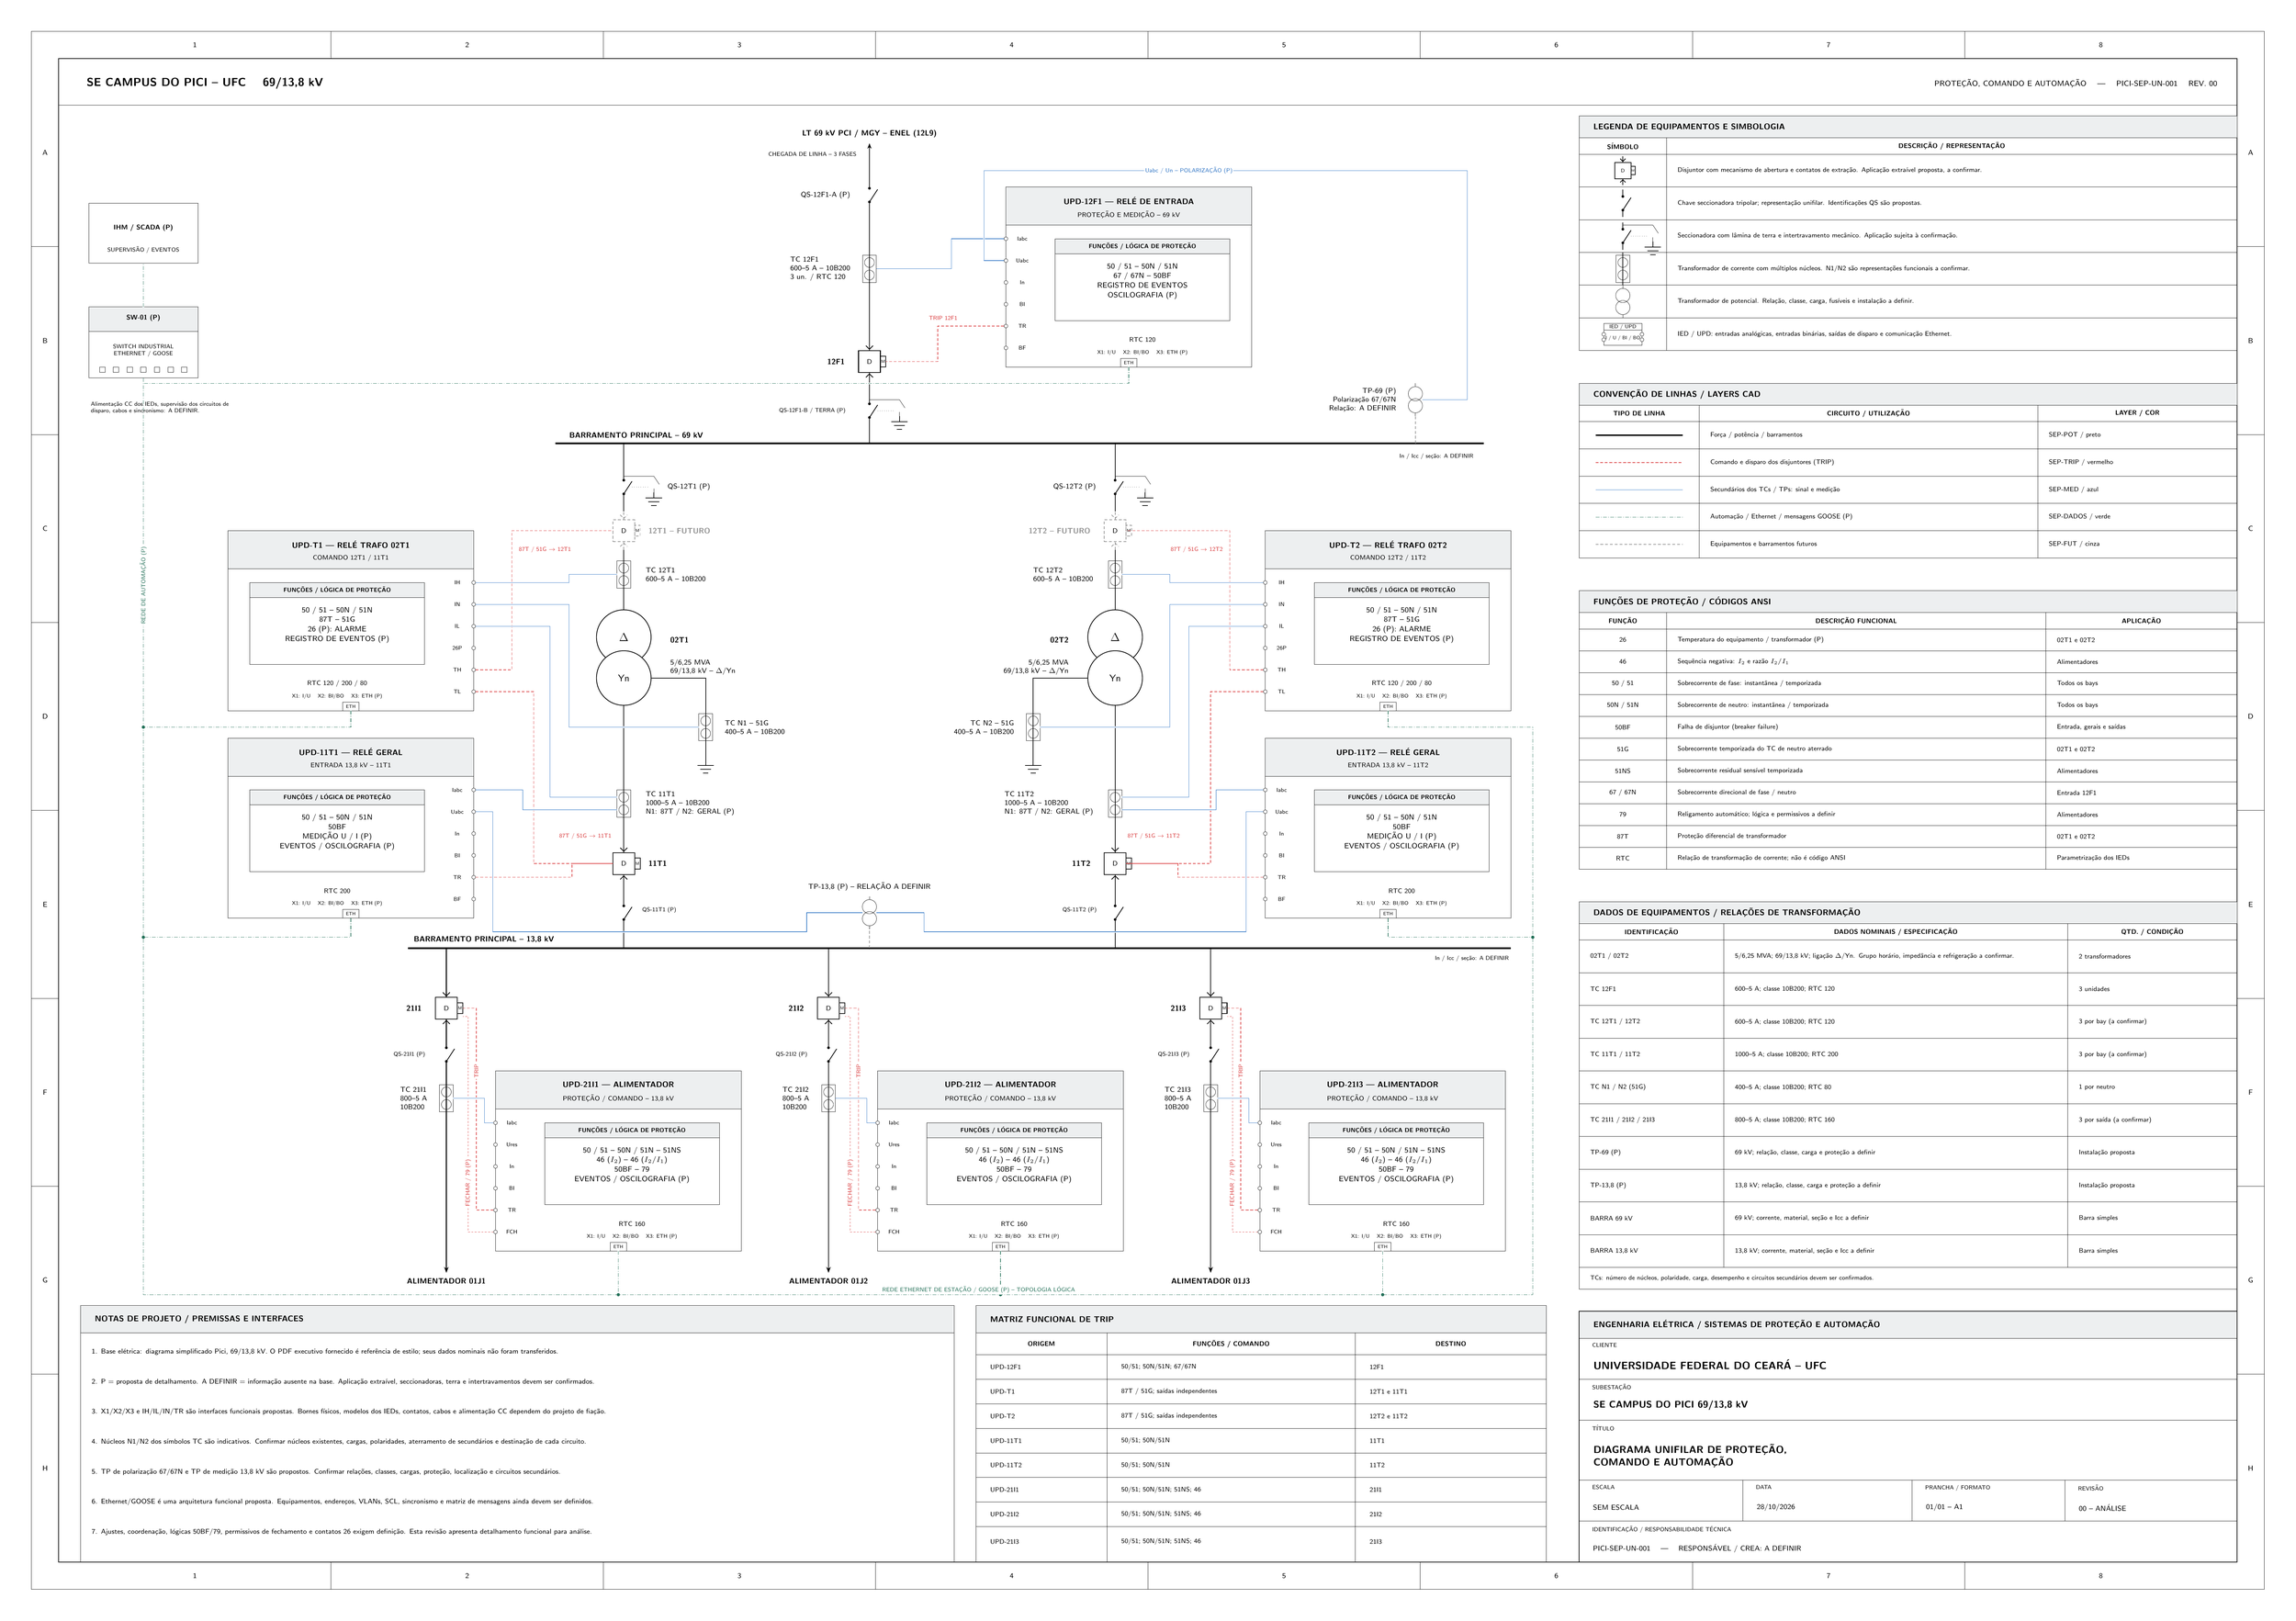
\begin{tikzpicture}[x=1mm,y=1mm,font=\fontsize{7.5}{9}\selectfont]
  \path[use as bounding box] (0,0) rectangle (834,587);

  % MOLDURA / GRID DE LOCALIZACAO 1--8 / A--H.
  \draw[linecad] (8,8) rectangle (826,579);
  \draw[power] (18,18) rectangle (816,569);
  \foreach \i in {1,...,8}{
    \pgfmathsetmacro{\xx}{18+(\i-.5)*99.75}
    \node at (\xx,574) {\i};
    \node at (\xx,13) {\i};
  }
  \foreach \i in {1,...,7}{
    \pgfmathsetmacro{\xx}{18+\i*99.75}
    \draw[linecad] (\xx,569)--(\xx,579) (\xx,8)--(\xx,18);
  }
  \foreach \letter[count=\i from 1] in {A,B,C,D,E,F,G,H}{
    \pgfmathsetmacro{\yy}{569-(\i-.5)*68.875}
    \node at (13,\yy) {\letter};
    \node at (821,\yy) {\letter};
  }
  \foreach \i in {1,...,7}{
    \pgfmathsetmacro{\yy}{569-\i*68.875}
    \draw[linecad] (8,\yy)--(18,\yy) (816,\yy)--(826,\yy);
  }
  \draw[linecad] (18,552)--(816,552);
  \node[anchor=west,font=\bfseries\fontsize{12}{14}\selectfont] at (27,560)
    {SE CAMPUS DO PICI -- UFC \quad 69/13,8 kV};
  \node[anchor=east,font=\fontsize{8}{10}\selectfont] at (810,560)
    {PROTEÇÃO, COMANDO E AUTOMAÇÃO \quad | \quad PICI-SEP-UN-001 \quad REV. 00};

  % CIRCUITO DE POTENCIA. Simbolos sobrepostos ocultam o condutor.
  \draw[power,-{Stealth[length=2mm]}] (315,428)--(315,538);
  \node[tag,anchor=south] at (315,539) {LT 69 kV PCI / MGY -- ENEL (12L9)};
  \node[tinycad,anchor=east] at (311,534) {CHEGADA DE LINHA -- 3 FASES};
  \draw[bus] (200,428)--(540,428);
  \node[tag,anchor=south west] at (204,429) {BARRAMENTO PRINCIPAL -- 69 kV};
  \node[tinycad,anchor=north east] at (537,425) {In / Icc / seção: A DEFINIR};
  \foreach \xx in {225,405}{\draw[power] (\xx,428)--(\xx,243);}
  \draw[bus] (146,243)--(550,243);
  \node[tag,anchor=south west] at (147,244) {BARRAMENTO PRINCIPAL -- 13,8 kV};
  \node[tinycad,anchor=north east] at (550,241) {In / Icc / seção: A DEFINIR};
  \draw[power] (225,342)--(255,342)--(255,312);
  \draw[power] (405,342)--(375,342)--(375,312);
  \CadEarth{255}{312}
  \CadEarth{375}{312}
  \foreach \xx in {160,300,440}{
    \draw[power,-{Stealth[length=2.2mm]}] (\xx,243)--(\xx,124);
  }

  % EQUIPAMENTOS DE LINHA E TPs PROPOSTOS.
  \CadQS{315}{519}{QS12F1A}
  \CadCT{315}{492}{TC12F1}
  \CadCB{315}{458}{DJ12F1}{normal}
  \CadQSEarth{315}{440}{QS12F1B}
  \node[labelcad,anchor=east] at (309,519) {QS-12F1-A (P)};
  \node[labelcad,anchor=east] at (309,492) {TC 12F1\\600--5 A -- 10B200\\3 un. / RTC 120};
  \node[tag,anchor=east] at (307,458) {12F1};
  \node[tinycad,anchor=east] at (307,440) {QS-12F1-B / TERRA (P)};
  \draw[future] (515,428)--(515,449);
  \CadTP{515}{444}{TP69}
  \node[labelcad,anchor=east,align=right] at (509,444) {TP-69 (P)\\Polarização 67/67N\\Relação: A DEFINIR};

  % BAYS DE TRANSFORMACAO.
  \foreach \xx/\nn in {225/1,405/2}{
    \CadQSEarth{\xx}{412}{QS12T\nn}
    \CadCB{\xx}{396}{DJ12T\nn}{future}
    \CadCT{\xx}{380}{TC12T\nn}
    \node[circle,draw=black,fill=white,line width=.75pt,minimum size=20mm,inner sep=0pt,
      font=\fontsize{12}{14}\selectfont] at (\xx,357) {$\Delta$};
    \node[circle,draw=black,fill=white,line width=.75pt,minimum size=20mm,inner sep=0pt,
      font=\fontsize{10}{12}\selectfont] at (\xx,342) {Yn};
    \CadCT{\xx}{296}{TC11T\nn}
    \CadCB{\xx}{274}{DJ11T\nn}{normal}
    \CadQS{\xx}{256}{QS11T\nn}
  }
  \CadCT{255}{324}{TCN1}
  \CadCT{375}{324}{TCN2}
  \node[labelcad,anchor=west] at (240,412) {QS-12T1 (P)};
  \node[labelcad,anchor=east] at (399,412) {QS-12T2 (P)};
  \node[tag,anchor=west,text=futuregray] at (233,396) {12T1 -- FUTURO};
  \node[tag,anchor=east,text=futuregray] at (397,396) {12T2 -- FUTURO};
  \node[labelcad,anchor=west] at (232,380) {TC 12T1\\600--5 A -- 10B200};
  \node[labelcad,anchor=east] at (398,380) {TC 12T2\\600--5 A -- 10B200};
  \node[tag,anchor=west] at (241,356) {02T1};
  \node[labelcad,anchor=west] at (241,346) {5/6,25 MVA\\69/13,8 kV -- $\Delta$/Yn};
  \node[tag,anchor=east] at (389,356) {02T2};
  \node[labelcad,anchor=east,align=right] at (389,346) {5/6,25 MVA\\69/13,8 kV -- $\Delta$/Yn};
  \node[labelcad,anchor=west] at (261,324) {TC N1 -- 51G\\400--5 A -- 10B200};
  \node[labelcad,anchor=east,align=right] at (369,324) {TC N2 -- 51G\\400--5 A -- 10B200};
  \node[labelcad,anchor=west] at (232,296) {TC 11T1\\1000--5 A -- 10B200\\N1: 87T / N2: GERAL (P)};
  \node[labelcad,anchor=east] at (398,296) {TC 11T2\\1000--5 A -- 10B200\\N1: 87T / N2: GERAL (P)};
  \node[tag,anchor=west] at (233,274) {11T1};
  \node[tag,anchor=east] at (397,274) {11T2};
  \node[tinycad,anchor=west] at (231,257) {QS-11T1 (P)};
  \node[tinycad,anchor=east] at (399,257) {QS-11T2 (P)};
  \draw[future] (315,243)--(315,261);
  \CadTP{315}{256}{TP138}
  \node[labelcad,anchor=south] at (315,263) {TP-13,8 (P) -- RELAÇÃO A DEFINIR};

  % IEDs: bornes funcionais, portas de rede e saídas independentes.
  \CadIED{EL}{365}{456}{UPD-12F1 | RELÉ DE ENTRADA}{PROTEÇÃO E MEDIÇÃO -- 69 kV}
    {50 / 51 -- 50N / 51N\\67 / 67N -- 50BF\\REGISTRO DE EVENTOS\\OSCILOGRAFIA (P)}{120}{0}
    {Iabc/I1/47,Uabc/I2/39,In/I3/31,BI/BI/23,TR/T1/15,BF/T2/7}
  \CadIED{T1}{80}{330}{UPD-T1 | RELÉ TRAFO 02T1}{COMANDO 12T1 / 11T1}
    {50 / 51 -- 50N / 51N\\87T -- 51G\\26 (P): ALARME\\REGISTRO DE EVENTOS (P)}{120 / 200 / 80}{1}
    {IH/I1/47,IN/I2/39,IL/I3/31,26P/BI/23,TH/T1/15,TL/T2/7}
  \CadIED{T2}{460}{330}{UPD-T2 | RELÉ TRAFO 02T2}{COMANDO 12T2 / 11T2}
    {50 / 51 -- 50N / 51N\\87T -- 51G\\26 (P): ALARME\\REGISTRO DE EVENTOS (P)}{120 / 200 / 80}{0}
    {IH/I1/47,IN/I2/39,IL/I3/31,26P/BI/23,TH/T1/15,TL/T2/7}
  \CadIED{G1}{80}{254}{UPD-11T1 | RELÉ GERAL}{ENTRADA 13,8 kV -- 11T1}
    {50 / 51 -- 50N / 51N\\50BF\\MEDIÇÃO U / I (P)\\EVENTOS / OSCILOGRAFIA (P)}{200}{1}
    {Iabc/I1/47,Uabc/I2/39,In/I3/31,BI/BI/23,TR/T1/15,BF/T2/7}
  \CadIED{G2}{460}{254}{UPD-11T2 | RELÉ GERAL}{ENTRADA 13,8 kV -- 11T2}
    {50 / 51 -- 50N / 51N\\50BF\\MEDIÇÃO U / I (P)\\EVENTOS / OSCILOGRAFIA (P)}{200}{0}
    {Iabc/I1/47,Uabc/I2/39,In/I3/31,BI/BI/23,TR/T1/15,BF/T2/7}

  % ALIMENTADORES: disjuntor, seccionamento, TC e IED.
  \foreach \xx/\ii/\ix in {160/1/178,300/2/318,440/3/458}{
    \CadCB{\xx}{221}{DJ21I\ii}{normal}
    \CadQS{\xx}{204}{QS21I\ii}
    \CadCT{\xx}{188}{TC21I\ii}
    \node[tag,anchor=east] at (\xx-8,221) {21I\ii};
    \node[tinycad,anchor=east] at (\xx-7,204) {QS-21I\ii\ (P)};
    \node[labelcad,anchor=east] at (\xx-6,188) {TC 21I\ii\\800--5 A\\10B200};
    \node[tag,anchor=north] at (\xx,123) {ALIMENTADOR 01J\ii};
    \CadIED{F\ii}{\ix}{132}{UPD-21I\ii\ | ALIMENTADOR}{PROTEÇÃO / COMANDO -- 13,8 kV}
      {50 / 51 -- 50N / 51N -- 51NS\\46 ($I_2$) -- 46 ($I_2/I_1$)\\50BF -- 79\\EVENTOS / OSCILOGRAFIA (P)}{160}{0}
      {Iabc/I1/47,Ures/I2/39,In/I3/31,BI/BI/23,TR/T1/15,FCH/T2/7}
  }

  % TRIP -- cada saida do rele de trafo e um contato independente.
  \draw[trip] (EL-T1)--(340,471)--(340,458)--(DJ12F1-TR);
  \node[triptag] at (342,474) {TRIP 12F1};
  \draw[trip] (T1-T1)--(184,345)--(184,396)--(221,396);
  \draw[trip] (T1-T2)--(192,337)--(192,274)--(221,274);
  \draw[trip] (G1-T1)--(206,269)--(206,274)--(221,274);
  \node[triptag,anchor=west] at (186,389) {87T / 51G $\rightarrow$ 12T1};
  \node[triptag,anchor=east] at (221,284) {87T / 51G $\rightarrow$ 11T1};
  \draw[trip] (T2-T1)--(447,345)--(447,396)--(409,396);
  \draw[trip] (T2-T2)--(440,337)--(440,274)--(409,274);
  \draw[trip] (G2-T1)--(428,269)--(428,274)--(409,274);
  \node[triptag,anchor=east] at (445,389) {87T / 51G $\rightarrow$ 12T2};
  \node[triptag,anchor=west] at (409,284) {87T / 51G $\rightarrow$ 11T2};
  \foreach \xx/\ii/\ix in {160/1/178,300/2/318,440/3/458}{
    \draw[trip] (F\ii-T1)--(\xx+11,147)--(\xx+11,221)--(DJ21I\ii-TR);
    \draw[control] (F\ii-T2)--(\xx+8,139)--(\xx+8,218)--(DJ21I\ii-CL);
    \node[triptag,rotate=90] at (\xx+11,198) {TRIP};
    \node[tinycad,rotate=90,fill=white,text=tripred] at (\xx+8,157) {FECHAR / 79 (P)};
  }

  % MEDICAO -- as linhas com halo nao conectam nos cruzamentos.
  \draw[signal] (TC12F1-E)--(345,492)--(345,503)--(EL-I1);
  \draw[signal] (TP69-E)--(534,444)--(534,528)--(357,528)--(357,495)--(EL-I2);
  \node[sigtag] at (432,528) {Uabc / Un -- POLARIZAÇÃO (P)};
  \draw[signal] (TC12T1-W)--(205,380)--(205,377)--(T1-I1);
  \draw[signal] (TCN1-W)--(205,324)--(205,369)--(T1-I2);
  % N1 e N2 propostos: circuitos separados para diferencial e geral.
  \draw[signal] (TC11T1-W1)--(198,298.3)--(198,361)--(T1-I3);
  \draw[signal] (TC11T1-W2)--(188,293.7)--(188,301)--(G1-I1);
  \draw[signal] (TC12T2-E)--(425,380)--(425,377)--(T2-I1);
  \draw[signal] (TCN2-E)--(425,324)--(425,369)--(T2-I2);
  \draw[signal] (TC11T2-E1)--(432,298.3)--(432,361)--(T2-I3);
  \draw[signal] (TC11T2-E2)--(442,293.7)--(442,301)--(G2-I1);
  \draw[signal] (TP138-W)--(292,256)--(292,249)--(177,249)--(177,293)--(G1-I2);
  \draw[signal] (TP138-E)--(335,256)--(335,249)--(453,249)--(453,293)--(G2-I2);
  \foreach \xx/\ii/\ix in {160/1/178,300/2/318,440/3/458}{
    \draw[signal] (TC21I\ii-E)--(\xx+14,188)--(\xx+14,179)--(F\ii-I1);
  }

  % REDE DE AUTOMACAO FUNCIONAL (P) -- sem afirmar GOOSE implementado.
  \draw[comm] (EL-NET)--(410,450)--(49,450)--(49,452);
  \draw[comm] (49,452)--(49,116)--(558,116)--(558,324);
  \draw[comm] (T1-NET)--(125,324)--(49,324);
  \draw[comm] (G1-NET)--(125,247)--(49,247);
  \draw[comm] (T2-NET)--(505,324)--(558,324);
  \draw[comm] (G2-NET)--(505,247)--(558,247);
  \foreach \ii/\xx in {1/223,2/363,3/503}{
    \draw[comm] (F\ii-NET)--(\xx,116);
    \node[netpoint] at (\xx,116) {};
  }
  \foreach \yy in {324,247}{\node[netpoint] at (49,\yy) {};}
  \node[netpoint] at (558,247) {};
  \node[nettag,anchor=south] at (355,116) {REDE ETHERNET DE ESTAÇÃO / GOOSE (P) -- TOPOLOGIA LÓGICA};
  \node[nettag,rotate=90] at (49,376) {REDE DE AUTOMAÇÃO (P)};
  \draw[linecad,fill=white] (29,452) rectangle (69,478);
  \fill[headerbg] (29.1,469) rectangle (68.9,477.9);
  \draw[linecad] (29,469)--(69,469);
  \node[font=\bfseries\fontsize{7}{8}\selectfont] at (49,474) {SW-01 (P)};
  \node[font=\fontsize{6}{7}\selectfont,align=center] at (49,462) {SWITCH INDUSTRIAL\\ETHERNET / GOOSE};
  \foreach \px in {34,39,44,49,54,59,64}{\draw[linecad] (\px-1,454) rectangle (\px+1,456);}
  \draw[comm] (49,478)--(49,494);
  \draw[linecad,fill=white] (29,494) rectangle (69,516);
  \node[font=\bfseries\fontsize{7}{8}\selectfont,align=center] at (49,507) {IHM / SCADA (P)};
  \node[font=\fontsize{6}{7}\selectfont,align=center] at (49,499) {SUPERVISÃO / EVENTOS};
  \node[tinycad,anchor=north west,text width=52mm] at (29,444)
    {Alimentação CC dos IEDs, supervisão dos circuitos de disparo, cabos e sincronismo: A DEFINIR.};

  % QUADROS LATERAIS -- incorporados no fonte para compilar isoladamente.
% Fragmento TikZ: quadros laterais. Coordenadas em milimetros.
% Area reservada: x=575..816, y=118..548. Selo abaixo de y=110.
\begin{scope}[font=\fontsize{6.8}{8}\selectfont]
  \tikzset{
    etitle/.style={font=\bfseries\fontsize{8.5}{10}\selectfont,anchor=west},
    ecol/.style={font=\bfseries\fontsize{6.8}{8}\selectfont,align=center},
    ecell/.style={anchor=west,align=left,inner sep=0pt},
    ecode/.style={align=center,inner sep=0pt}
  }

  % 01 -- LEGENDA DE EQUIPAMENTOS E SIMBOLOGIA.
  \fill[headerbg] (575,540) rectangle (816,548);
  \draw[linecad] (575,462) rectangle (816,548);
  \foreach \y in {540,534,522,510,498,486,474}{
    \draw[linecad] (575,\y) -- (816,\y);
  }
  \draw[linecad] (607,462) -- (607,540);
  \node[etitle] at (579,544) {LEGENDA DE EQUIPAMENTOS E SIMBOLOGIA};
  \node[ecol] at (591,537) {SÍMBOLO};
  \node[ecol] at (711.5,537) {DESCRIÇÃO / REPRESENTAÇÃO};

  \begin{scope}[shift={(591,528)},scale=.75,transform shape]
    \CadCB{0}{0}{LEGCBA}{normal}
  \end{scope}
  \node[ecell,text width=198mm] at (611,528)
    {Disjuntor com mecanismo de abertura e contatos de extração. Aplicação extraível proposta, a confirmar.};
  \CadQS{591}{516}{LEGQSA}
  \node[ecell,text width=198mm] at (611,516)
    {Chave seccionadora tripolar; representação unifilar. Identificações QS são propostas.};
  \CadQSEarth{591}{504}{LEGQST}
  \node[ecell,text width=198mm] at (611,504)
    {Seccionadora com lâmina de terra e intertravamento mecânico. Aplicação sujeita à confirmação.};
  \CadCT{591}{492}{LEGCTA}
  \node[ecell,text width=198mm] at (611,492)
    {Transformador de corrente com múltiplos núcleos. N1/N2 são representações funcionais a confirmar.};
  \CadTP{591}{480}{LEGTPA}
  \node[ecell,text width=198mm] at (611,480)
    {Transformador de potencial. Relação, classe, carga, fusíveis e instalação a definir.};
  \CadIEDLegend{591}{468}
  \node[ecell,text width=198mm] at (611,468)
    {IED / UPD: entradas analógicas, entradas binárias, saídas de disparo e comunicação Ethernet.};

  % 02 -- CONVENCAO DE LINHAS / LAYERS CAD.
  \fill[headerbg] (575,442) rectangle (816,450);
  \draw[linecad] (575,386) rectangle (816,450);
  \foreach \y in {442,436,426,416,406,396}{
    \draw[linecad] (575,\y) -- (816,\y);
  }
  \draw[linecad] (619,386) -- (619,442);
  \draw[linecad] (743,386) -- (743,442);
  \node[etitle] at (579,446) {CONVENÇÃO DE LINHAS / LAYERS CAD};
  \node[ecol] at (597,439) {TIPO DE LINHA};
  \node[ecol] at (681,439) {CIRCUITO / UTILIZAÇÃO};
  \node[ecol] at (779.5,439) {LAYER / COR};
  \draw[bus] (581,431) -- (613,431);
  \draw[trip] (581,421) -- (613,421);
  \draw[signal] (581,411) -- (613,411);
  \draw[comm] (581,401) -- (613,401);
  \draw[future] (581,391) -- (613,391);
  \node[ecell] at (623,431) {Força / potência / barramentos};
  \node[ecell] at (623,421) {Comando e disparo dos disjuntores (TRIP)};
  \node[ecell] at (623,411) {Secundários dos TCs / TPs: sinal e medição};
  \node[ecell] at (623,401) {Automação / Ethernet / mensagens GOOSE (P)};
  \node[ecell] at (623,391) {Equipamentos e barramentos futuros};
  \node[ecell] at (747,431) {SEP-POT / preto};
  \node[ecell] at (747,421) {SEP-TRIP / vermelho};
  \node[ecell] at (747,411) {SEP-MED / azul};
  \node[ecell] at (747,401) {SEP-DADOS / verde};
  \node[ecell] at (747,391) {SEP-FUT / cinza};

  % 03 -- FUNCOES DE PROTECAO.
  \fill[headerbg] (575,366) rectangle (816,374);
  \draw[linecad] (575,272) rectangle (816,374);
  \foreach \y in {366,360,352,344,336,328,320,312,304,296,288,280}{
    \draw[linecad] (575,\y) -- (816,\y);
  }
  \draw[linecad] (607,272) -- (607,366);
  \draw[linecad] (746,272) -- (746,366);
  \node[etitle] at (579,370) {FUNÇÕES DE PROTEÇÃO / CÓDIGOS ANSI};
  \node[ecol] at (591,363) {FUNÇÃO};
  \node[ecol] at (676.5,363) {DESCRIÇÃO FUNCIONAL};
  \node[ecol] at (781,363) {APLICAÇÃO};
  \foreach \code/\desc/\appl/\y in {
    {26}/{Temperatura do equipamento / transformador (P)}/{02T1 e 02T2}/356,
    {46}/{Sequência negativa: $I_2$ e razão $I_2/I_1$}/{Alimentadores}/348,
    {50 / 51}/{Sobrecorrente de fase: instantânea / temporizada}/{Todos os bays}/340,
    {50N / 51N}/{Sobrecorrente de neutro: instantânea / temporizada}/{Todos os bays}/332,
    {50BF}/{Falha de disjuntor (breaker failure)}/{Entrada, gerais e saídas}/324,
    {51G}/{Sobrecorrente temporizada do TC de neutro aterrado}/{02T1 e 02T2}/316,
    {51NS}/{Sobrecorrente residual sensível temporizada}/{Alimentadores}/308,
    {67 / 67N}/{Sobrecorrente direcional de fase / neutro}/{Entrada 12F1}/300,
    {79}/{Religamento automático; lógica e permissivos a definir}/{Alimentadores}/292,
    {87T}/{Proteção diferencial de transformador}/{02T1 e 02T2}/284,
    {RTC}/{Relação de transformação de corrente; não é código ANSI}/{Parametrização dos IEDs}/276
  }{
    \node[ecode] at (591,\y) {\code};
    \node[ecell] at (611,\y) {\desc};
    \node[ecell] at (750,\y) {\appl};
  }

  % 04 -- DADOS DOS TRANSFORMADORES, TRANSFORMADORES DE INSTRUMENTO E BARRAS.
  \fill[headerbg] (575,252) rectangle (816,260);
  \draw[linecad] (575,118) rectangle (816,260);
  \foreach \y in {252,246,234,222,210,198,186,174,162,150,138,126}{
    \draw[linecad] (575,\y) -- (816,\y);
  }
  \draw[linecad] (628,126) -- (628,252);
  \draw[linecad] (754,126) -- (754,252);
  \node[etitle] at (579,256) {DADOS DE EQUIPAMENTOS / RELAÇÕES DE TRANSFORMAÇÃO};
  \node[ecol] at (601.5,249) {IDENTIFICAÇÃO};
  \node[ecol] at (691,249) {DADOS NOMINAIS / ESPECIFICAÇÃO};
  \node[ecol] at (785,249) {QTD. / CONDIÇÃO};

  \node[ecell] at (579,240) {02T1 / 02T2};
  \node[ecell,text width=119mm] at (632,240)
    {5/6,25 MVA; 69/13,8 kV; ligação $\Delta$/Yn. Grupo horário, impedância e refrigeração a confirmar.};
  \node[ecell] at (758,240) {2 transformadores};

  \node[ecell] at (579,228) {TC 12F1};
  \node[ecell] at (632,228) {600--5 A; classe 10B200; RTC 120};
  \node[ecell] at (758,228) {3 unidades};

  \node[ecell] at (579,216) {TC 12T1 / 12T2};
  \node[ecell] at (632,216) {600--5 A; classe 10B200; RTC 120};
  \node[ecell] at (758,216) {3 por bay (a confirmar)};

  \node[ecell] at (579,204) {TC 11T1 / 11T2};
  \node[ecell] at (632,204) {1000--5 A; classe 10B200; RTC 200};
  \node[ecell] at (758,204) {3 por bay (a confirmar)};

  \node[ecell] at (579,192) {TC N1 / N2 (51G)};
  \node[ecell] at (632,192) {400--5 A; classe 10B200; RTC 80};
  \node[ecell] at (758,192) {1 por neutro};

  \node[ecell] at (579,180) {TC 21I1 / 21I2 / 21I3};
  \node[ecell] at (632,180) {800--5 A; classe 10B200; RTC 160};
  \node[ecell] at (758,180) {3 por saída (a confirmar)};

  \node[ecell] at (579,168) {TP-69 (P)};
  \node[ecell] at (632,168) {69 kV; relação, classe, carga e proteção a definir};
  \node[ecell] at (758,168) {Instalação proposta};

  \node[ecell] at (579,156) {TP-13,8 (P)};
  \node[ecell] at (632,156) {13,8 kV; relação, classe, carga e proteção a definir};
  \node[ecell] at (758,156) {Instalação proposta};

  \node[ecell] at (579,144) {BARRA 69 kV};
  \node[ecell] at (632,144) {69 kV; corrente, material, seção e Icc a definir};
  \node[ecell] at (758,144) {Barra simples};

  \node[ecell] at (579,132) {BARRA 13,8 kV};
  \node[ecell] at (632,132) {13,8 kV; corrente, material, seção e Icc a definir};
  \node[ecell] at (758,132) {Barra simples};

  \node[ecell,font=\fontsize{6.4}{7.5}\selectfont] at (579,122)
    {TCs: número de núcleos, polaridade, carga, desempenho e circuitos secundários devem ser confirmados.};
\end{scope}


  % NOTAS DE PROJETO -- inferior esquerdo.
  \draw[linecad] (26,18) rectangle (346,112);
  \fill[headerbg] (26.1,102) rectangle (345.9,111.9);
  \draw[linecad] (26,102)--(346,102);
  \node[anchor=west,font=\bfseries\fontsize{8.5}{10}\selectfont] at (30,107)
    {NOTAS DE PROJETO / PREMISSAS E INTERFACES};
  \foreach \yy/\txt in {
    95/{1. Base elétrica: diagrama simplificado Pici, 69/13,8 kV. O PDF executivo fornecido é referência de estilo; seus dados nominais não foram transferidos.},
    84/{2. P = proposta de detalhamento. A DEFINIR = informação ausente na base. Aplicação extraível, seccionadoras, terra e intertravamentos devem ser confirmados.},
    73/{3. X1/X2/X3 e IH/IL/IN/TR são interfaces funcionais propostas. Bornes físicos, modelos dos IEDs, contatos, cabos e alimentação CC dependem do projeto de fiação.},
    62/{4. Núcleos N1/N2 dos símbolos TC são indicativos. Confirmar núcleos existentes, cargas, polaridades, aterramento de secundários e destinação de cada circuito.},
    51/{5. TP de polarização 67/67N e TP de medição 13,8 kV são propostos. Confirmar relações, classes, cargas, proteção, localização e circuitos secundários.},
    40/{6. Ethernet/GOOSE é uma arquitetura funcional proposta. Equipamentos, endereços, VLANs, SCL, sincronismo e matriz de mensagens ainda devem ser definidos.},
    29/{7. Ajustes, coordenação, lógicas 50BF/79, permissivos de fechamento e contatos 26 exigem definição. Esta revisão apresenta detalhamento funcional para análise.}
  }{
    \node[anchor=west,align=left,text width=309mm,font=\fontsize{7.2}{8.6}\selectfont,inner sep=0pt] at (30,\yy) {\txt};
  }

  % MATRIZ FUNCIONAL DE DISPAROS CONFIRMADOS NA TOPOLOGIA.
  \draw[linecad] (354,18) rectangle (563,112);
  \fill[headerbg] (354.1,102) rectangle (562.9,111.9);
  \node[anchor=west,font=\bfseries\fontsize{8.5}{10}\selectfont] at (358,107) {MATRIZ FUNCIONAL DE TRIP};
  \foreach \yy in {102,94,85,76,67,58,49,40,31}{\draw[linecad] (354,\yy)--(563,\yy);}
  \draw[linecad] (402,18)--(402,102) (493,18)--(493,102);
  \node[font=\bfseries\fontsize{6.8}{8}\selectfont] at (378,98) {ORIGEM};
  \node[font=\bfseries\fontsize{6.8}{8}\selectfont] at (447.5,98) {FUNÇÕES / COMANDO};
  \node[font=\bfseries\fontsize{6.8}{8}\selectfont] at (528,98) {DESTINO};
  \foreach \src/\fun/\dst/\yy in {
    {UPD-12F1}/{50/51; 50N/51N; 67/67N}/{12F1}/89.5,
    {UPD-T1}/{87T / 51G; saídas independentes}/{12T1 e 11T1}/80.5,
    {UPD-T2}/{87T / 51G; saídas independentes}/{12T2 e 11T2}/71.5,
    {UPD-11T1}/{50/51; 50N/51N}/{11T1}/62.5,
    {UPD-11T2}/{50/51; 50N/51N}/{11T2}/53.5,
    {UPD-21I1}/{50/51; 50N/51N; 51NS; 46}/{21I1}/44.5,
    {UPD-21I2}/{50/51; 50N/51N; 51NS; 46}/{21I2}/35.5
  }{
    \node[anchor=west,font=\fontsize{6.8}{8}\selectfont] at (358,\yy) {\src};
    \node[anchor=west,font=\fontsize{6.8}{8}\selectfont] at (406,\yy) {\fun};
    \node[anchor=west,font=\fontsize{6.8}{8}\selectfont] at (497,\yy) {\dst};
  }
  \node[anchor=west,font=\fontsize{6.8}{8}\selectfont] at (358,25.5) {UPD-21I3};
  \node[anchor=west,font=\fontsize{6.8}{8}\selectfont] at (406,25.5) {50/51; 50N/51N; 51NS; 46};
  \node[anchor=west,font=\fontsize{6.8}{8}\selectfont] at (497,25.5) {21I3};

  % SELO DE ENGENHARIA -- inferior direito.
  \draw[power] (575,18) rectangle (816,110);
  \foreach \yy in {100,85,70,48,33}{\draw[linecad] (575,\yy)--(816,\yy);}
  \fill[headerbg] (575.2,100.1) rectangle (815.8,109.8);
  \node[anchor=west,font=\bfseries\fontsize{8.5}{10}\selectfont] at (579,105)
    {ENGENHARIA ELÉTRICA / SISTEMAS DE PROTEÇÃO E AUTOMAÇÃO};
  \node[tinycad,anchor=north west] at (579,99) {CLIENTE};
  \node[anchor=west,font=\bfseries\fontsize{11}{13}\selectfont] at (579,90.5)
    {UNIVERSIDADE FEDERAL DO CEARÁ -- UFC};
  \node[tinycad,anchor=north west] at (579,84) {SUBESTAÇÃO};
  \node[anchor=west,font=\bfseries\fontsize{10}{12}\selectfont] at (579,75.5)
    {SE CAMPUS DO PICI 69/13,8 kV};
  \node[tinycad,anchor=north west] at (579,69) {TÍTULO};
  \node[anchor=west,font=\bfseries\fontsize{10.5}{13}\selectfont,align=left] at (579,57)
    {DIAGRAMA UNIFILAR DE PROTEÇÃO,\\COMANDO E AUTOMAÇÃO};
  \draw[linecad] (635,33)--(635,48) (697,33)--(697,48) (753,33)--(753,48);
  \node[tinycad,anchor=north west] at (579,47) {ESCALA};
  \node[labelcad,anchor=west] at (579,38) {SEM ESCALA};
  \node[tinycad,anchor=north west] at (639,47) {DATA};
  \node[labelcad,anchor=west] at (639,38) {28/10/2026};
  \node[tinycad,anchor=north west] at (701,47) {PRANCHA / FORMATO};
  \node[labelcad,anchor=west] at (701,38) {01/01 -- A1};
  \node[tinycad,anchor=north west] at (757,47) {REVISÃO};
  \node[labelcad,anchor=west] at (757,38) {00 -- ANÁLISE};
  \node[tinycad,anchor=north west] at (579,32) {IDENTIFICAÇÃO / RESPONSABILIDADE TÉCNICA};
  \node[labelcad,anchor=west] at (579,23) {PICI-SEP-UN-001 \quad | \quad RESPONSÁVEL / CREA: A DEFINIR};
\end{tikzpicture}
\end{document}
